% Provenance (never printed): see sources/outline_sources.md (Year 3: the
% structure of the Galaxy; the rotation curve and dark matter; galaxy types;
% the distance ladder, Hubble's law recalled from the physics books).
% Brief: sources/book5/BRIEFS.md, ch. 29. Curves from figdata/bachelor-3/
% rotation_curve.py (the circular velocity curve of Eilers et al. 2019 with the
% Pouliasis et al. 2017 Model I baryons and an NFW halo fitted to it) and
% distance_ladder.py (the OGLE-IV Cepheids of the Large Magellanic Cloud, CDS
% J/AcA/65/297, and the ranges of the rungs). Exercise and problem values in the
% Book 5 scratch calculator calc/ch29.py. The survey of Part I of the problem and
% the galaxies of the exercises are invented.
\chapter{The Milky Way and Galaxies}\label{ch:b3:milky-way-galaxies}

In the Solar System, the planets far from the Sun move slowly: Mercury
circles it at \qty{47.4}{km.s^{-1}}, Neptune at \qty{5.4}{km.s^{-1}}, as
Kepler's third law requires of bodies held by one central mass. The stars
of the Galaxy do not behave that way. Measured from the motions of more
than twenty thousand red giants, the speed of their circular orbits is
\qty{227}{km.s^{-1}} at \qty{5}{kpc} from the centre, \qty{229}{km.s^{-1}}
at the Sun, and still \qty{198}{km.s^{-1}} at \qty{25}{kpc}, where hardly
any stars or gas remain. If the mass we see were all there is, the outer
stars would be far slower. Something unseen holds them. This chapter
describes the Galaxy we live in, weighs it from its rotation, sorts the
other galaxies into types, and climbs the chain of methods by which their
distances, and the expansion of the Universe, are measured.
% ledger: planet:Mercury.vorb, planet:Neptune.vorb, eilers19:vc, eilers19:table1

\begin{recall}
The Milky Way, the Doppler effect, Kepler's laws, Newton's theorem on the
attraction of a spherical shell, dark matter, black holes and their
Schwarzschild radius, supernovae, white dwarfs, the 21-cm line of atomic
hydrogen and Hubble's law are in the physics books. The annual parallax,
the parsec, flux and luminosity, apparent and absolute magnitudes, the
distance modulus, photometric bands and the colour index are in the
Year~1 volume, in its chapter on telescopes and photometry. The
interstellar medium and its dust are in the Year~2 volume, in its chapter
on the interstellar medium and star formation.
\end{recall}

\section{The structure of the Galaxy}\label{sec:b3:milky-way-galaxies:structure}

Seen from the Earth, the Galaxy is the Milky Way: a band of light around
the whole sky, crossed by dark lanes of dust and brightest towards the
constellation Sagittarius, where its centre lies. The band is the disc in
which the Sun sits, seen edge-on from inside.

\begin{omfigure}
\centering
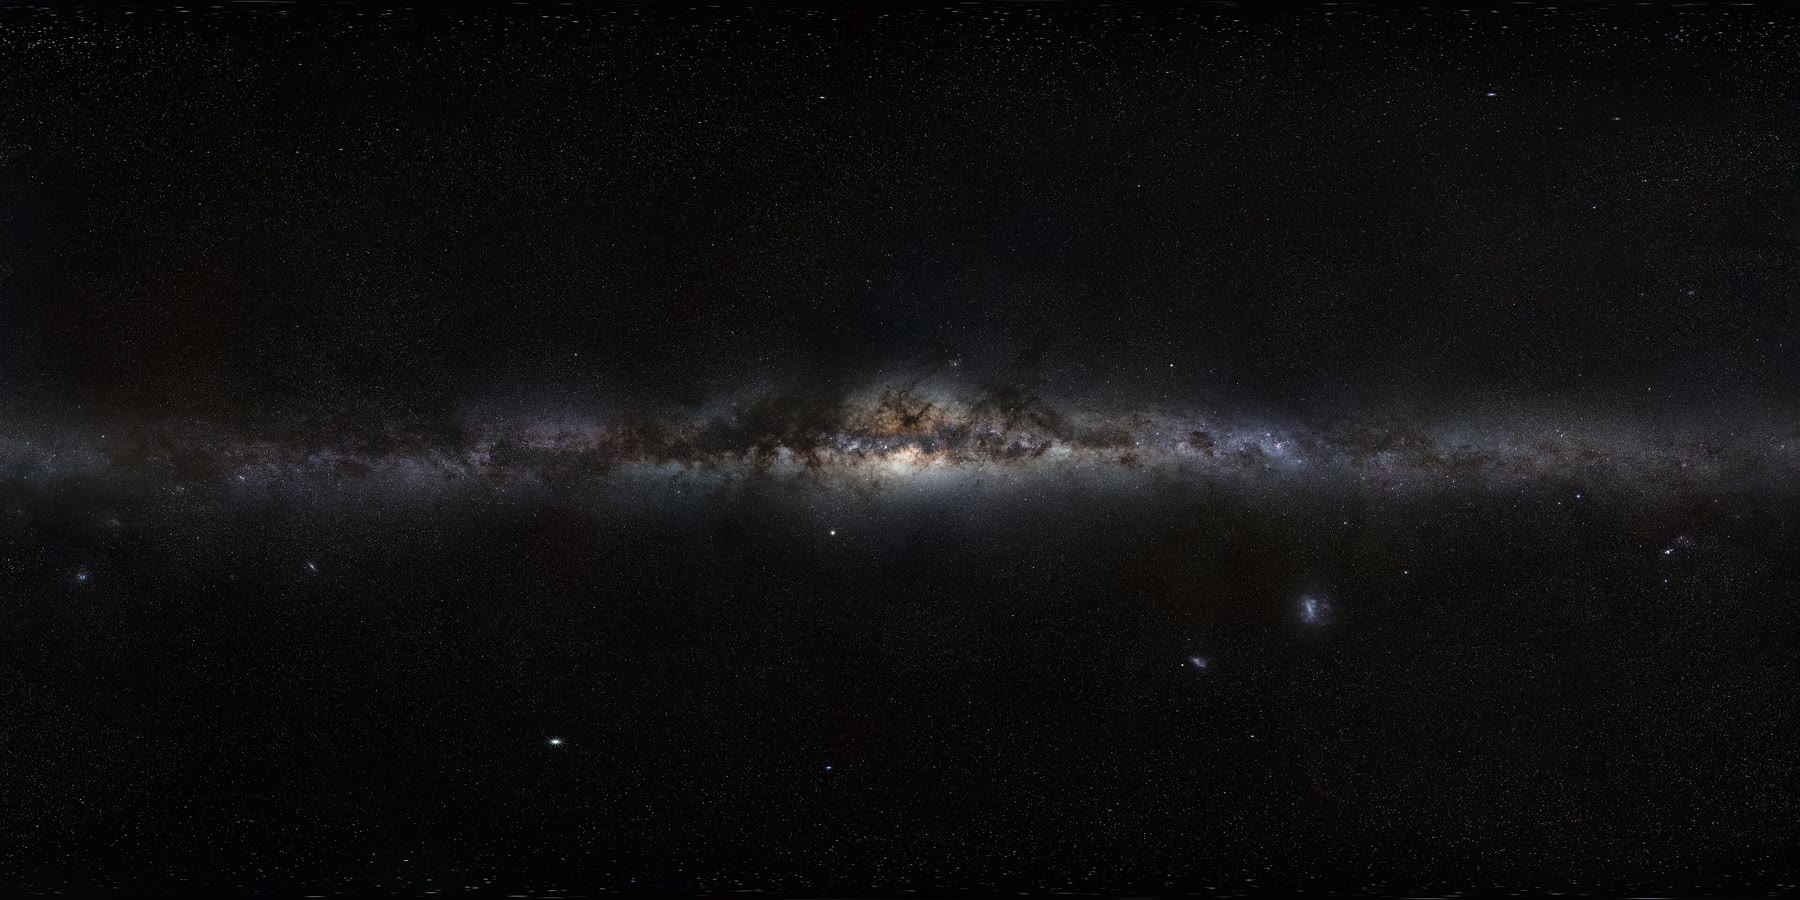
\includegraphics[width=0.96\linewidth]{images/book5/b3-milky-way-panorama.jpg}
\par\smallskip{\small The whole sky in one image, projected so that the
plane of the Galaxy runs across the middle and its centre lies at the
centre of the picture. The band is the disc seen from inside; the dark
lanes are dust in the disc, hiding the stars behind it; the central bulge
swells around the centre. The two small patches below the band, on the
right, are the Large and Small Magellanic Clouds, two satellite galaxies;
the faint smudge below the band near the left edge is the Andromeda
galaxy. Photograph ESO/S.~Brunier, CC BY~4.0.}\label{fig:b3:milky-way-galaxies:panorama}
\end{omfigure}
% ledger: photo:b3-milky-way-panorama, mcconn12:local-group

\begin{definition}[Galactic disc, thick disc, bulge and stellar halo]\label{def:b3:milky-way-galaxies:structure}
The \emph{Galactic disc}\index{Galactic disc} is the flattened component of
the Galaxy, made of stars, gas and dust in nearly circular orbits about its
centre; its density falls off roughly exponentially with height above its
mid-plane and with distance from its centre, over a scale height and a
scale length. The \emph{thick disc}\index{thick disc} is a second, older
disc component of larger scale height and smaller mass. The
\emph{Galactic bulge}\index{Galactic bulge} is the central concentration of
stars that swells out of the disc. The \emph{stellar halo}\index{stellar
halo} is the sparse, roughly spheroidal component of old stars and
globular clusters that surrounds the disc and the bulge.
\end{definition}

The Galaxy is a barred spiral. In the neighbourhood of the Sun the thin
disc has a scale height of about \qty{300}{pc} and the \omterm{def:b3:milky-way-galaxies:structure}{thick disc} of
about \qty{900}{pc}; their scale lengths are about \qty{2.6}{kpc} and
\qty{2.0}{kpc}. The \omterm{def:b3:milky-way-galaxies:structure}{thick disc} holds some \qty{6e9}{} solar masses,
roughly a fifth of the thin disc. Seen from the side, the bulge is a box
or a peanut: it is the thickened inner part of a bar of stars about
\qty{5}{kpc} in half-length, whose long axis makes an angle of
\ang{27} with the line from the Sun to the centre. The \omterm{def:b3:milky-way-galaxies:structure}{stellar halo} holds
only about one percent of the stars. All together, the stars of the Galaxy
weigh about \qty{5e10}{} solar masses.
% ledger: bhg16:structure

\begin{omfigure}
\centering
\begin{tikzpicture}[x=0.17cm, y=0.17cm, font=\scriptsize]
% edge-on view
\begin{scope}
\fill[omProp!8] (0,0) circle (17);
\draw[omProp!60, densely dotted] (0,0) circle (17);
\fill[black!12] (0,0) ellipse (15 and 2.4);
\fill[black!30] (0,0) ellipse (15 and 0.8);
\fill[black!45] (-3.2,0) .. controls (-3.4,2.3) and (-1.2,2.0) .. (0,1.4)
  .. controls (1.2,2.0) and (3.4,2.3) .. (3.2,0)
  .. controls (3.4,-2.3) and (1.2,-2.0) .. (0,-1.4)
  .. controls (-1.2,-2.0) and (-3.4,-2.3) .. (-3.2,0) -- cycle;
\foreach \p in {(-10,9),(6,12),(12,-7),(-6,-13),(-13,-4),(3,-9),(12,8)}
  \fill[omProp] \p circle (0.35);
\fill[ocYellow, draw=black] (-8.2,0.15) circle (0.55);
\node[anchor=south] at (-8.2,0.9) {Sun};
\draw[|<->|] (0,-4.6) -- node[below] {$R_0 \approx \qty{8.2}{kpc}$} (-8.2,-4.6);
\node[anchor=west] at (15.3,0) {thin disc};
\node[anchor=west] at (13.2,2.8) {thick disc};
\draw[->] (4.6,4.6) node[anchor=south west, inner sep=1pt] {bulge} -- (2.4,1.7);
\node[omProp!80!black] at (-11,13.5) {stellar halo};
\node at (0,-19.5) {(a) seen edge-on};
\end{scope}
% face-on view
\begin{scope}[xshift=7.6cm]
\fill[omProp!8] (0,0) circle (17);
\draw[omProp!60, densely dotted] (0,0) circle (17);
\fill[black!12] (0,0) circle (15);
\foreach \a in {0,180} {
  \draw[line width=1.6pt, black!40, rotate=\a+63]
    plot[domain=0:3.9, samples=50] ({5*exp(0.25*\x)*cos(\x r)}, {5*exp(0.25*\x)*sin(\x r)});
}
\fill[black!45, rotate=63] (0,0) ellipse (5 and 1.5);
\draw[dashed] (0,0) circle (8.2);
\fill[ocYellow, draw=black] (0,-8.2) circle (0.55);
\node[anchor=north] at (0,-8.9) {Sun};
\draw[dotted, thick] (0,0) -- (0,-8.2);
\draw[thick, ->] (0,0) ++(25:16) arc (25:-25:16);
\node[anchor=west] at (17.3,0) {rotation};
\node[anchor=west, fill=black!12, inner sep=1pt] at (3.4,3.4) {bar};
\draw[|-|] (6,-15.5) -- node[below] {\qty{5}{kpc}} (11,-15.5);
\node at (0,-19.5) {(b) seen from the north Galactic pole};
\end{scope}
\end{tikzpicture}
\par\smallskip{\small A sketch of the Galaxy, to scale for its main
dimensions. (a)~Edge-on: the thin disc (dark band), the \omterm{def:b3:milky-way-galaxies:structure}{thick disc} (light
band), the box-shaped bulge, and the \omterm{def:b3:milky-way-galaxies:structure}{stellar halo} with its globular
clusters (orange dots); the Sun lies in the disc, about \qty{8.2}{kpc}
from the centre and about \qty{25}{pc} above the mid-plane (too small to
show). (b)~Seen from the north Galactic pole: the bar, about
\qty{5}{kpc} in half-length, tilted by \ang{27} to the line from the Sun
to the centre (dotted); the solar circle (dashed); spiral arms drawn
schematically; the Galaxy turns clockwise in this view.}\label{fig:b3:milky-way-galaxies:sketch}
\end{omfigure}
% ledger: bhg16:structure, gravity19:r0

\begin{definition}[Stellar population]\label{def:b3:milky-way-galaxies:populations}
A \emph{stellar population}\index{stellar population} is a group of stars
of a galaxy that share a range of ages, of chemical compositions and of
orbits. The young stars of the thin disc, rich in elements heavier than
helium and on nearly circular orbits, are traditionally called
population~I; the old stars of the halo and of the globular clusters, poor
in heavy elements and on orbits of large random motions with little net
rotation, population~II.
\end{definition}

The \omterm{def:b3:milky-way-galaxies:structure}{thick disc} lies in between: its stars are mostly older than those of
the thin disc and, at a given iron content, richer in the light elements
that astronomers call alpha elements, measured relative to iron. The
\omterm{def:b3:milky-way-galaxies:structure}{stellar halo} is a
fossil record: much of it was assembled from small galaxies that fell into
the Galaxy and were torn apart by its tides, and some of their streams of
stars can still be followed across the sky.
% ledger: bhg16:populations

\begin{definition}[Galactic coordinates]\label{def:b3:milky-way-galaxies:coordinates}
The \emph{Galactic coordinates}\index{Galactic coordinates} of a direction
are its \emph{Galactic latitude} $b$, the angle from the Galactic plane
(positive towards the north Galactic pole), and its \emph{Galactic
longitude} $\ell$, measured in the plane from the direction of the
Galactic Centre ($\ell = 0$) through $\ell = \ang{90}$, the direction
towards which the Galaxy's rotation carries the Sun. The plane was
defined in 1958 as the principal plane of the Galaxy's atomic hydrogen;
the north Galactic pole lies at right ascension \ang{192.25}
($12^\mathrm{h}49^\mathrm{m}$) and declination \ang{27.4} (equinox
1950).
\end{definition}
% ledger: liu11:galactic, reid20:sgra

The Sun is not quite in the plane: it lies some \qty{25}{pc} north of it.
Its distance from the centre, $R_0$, was long the most uncertain number of
Galactic astronomy. It is now measured geometrically: the star S2 circles
the central black hole of the Galaxy on a \num{16}-year orbit, whose
angular size on the sky and velocity along the line of sight, followed
for 27 years, give the distance to the centre directly:
$R_0 = \qty{8178}{pc}$, with a statistical error of \qty{13}{pc} and a
systematic one of \qty{22}{pc}. A review of all methods gives
$R_0 = \qty[separate-uncertainty=true]{8.2 \pm 0.1}{kpc}$.
% ledger: bhg16:structure, gravity19:r0

\section{Rotation and the dark halo}\label{sec:b3:milky-way-galaxies:rotation}

\begin{definition}[Local standard of rest]\label{def:b3:milky-way-galaxies:lsr}
The \emph{local standard of rest}\index{local standard of rest} (LSR) is
the frame of reference that moves on the circular orbit about the Galactic
Centre passing through the Sun's present position. Velocities of nearby
stars and gas are quoted relative to it.
\end{definition}

The Sun moves relative to the LSR by about \qty{10}{km.s^{-1}} towards the
Galactic Centre, \qty{11}{km.s^{-1}} in the direction of rotation and
\qty{7}{km.s^{-1}} towards the north Galactic pole: a small peculiar
motion on top of an orbit at a speed $V_0$ of a few hundred kilometres
per second. Seen from the Earth, the radio source at the centre of the
Galaxy drifts along the Galactic plane by \qty{6.411}{mas} a year; nearly
all of that drift is the reflex of the Sun's orbit, and it gives the Sun's
total speed about the centre, \qty[separate-uncertainty=true]{248 \pm 3}{km.s^{-1}}
(\cref{exo:b3:milky-way-galaxies:2}).
% ledger: bhg16:lsr, reid20:sgra

\begin{definition}[Rotation curve; Oort constants]\label{def:b3:milky-way-galaxies:rotation-curve}
The \emph{rotation curve}\index{rotation curve} of a disc galaxy is the
speed $V(R)$ of a circular orbit in its plane as a function of the
distance $R$ from its centre. For the Galaxy, with $V_0 = V(R_0)$ and
$V'_0 = \mathrm{d}V/\mathrm{d}R$ at $R_0$, the \emph{Oort
constants}\index{Oort constants} are
\[
A = \frac12\left(\frac{V_0}{R_0} - V'_0\right), \qquad
B = -\frac12\left(\frac{V_0}{R_0} + V'_0\right).
\]
\end{definition}

$A$ measures the shear of the disc's rotation and $B$ its vorticity: in a
disc turning as a solid body $V'_0 = V_0/R_0$ and $A = 0$; on a flat
\omterm{def:b3:milky-way-galaxies:rotation-curve}{rotation curve} $A = -B$. Their difference is the angular speed of the LSR,
$A - B = V_0/R_0 = \omega_0$, and their sum the slope, $A + B = -V'_0$.

\begin{theorem}[Oort's formulas]\label{thm:b3:milky-way-galaxies:oort}
A star at a distance $d \ll R_0$ from the Sun, in the Galactic plane at
longitude $\ell$, on a circular orbit, has relative to the LSR the radial
velocity $v_r$ and the transverse velocity $v_t$ (positive in the
direction of increasing $\ell$)
\[
v_r = A\,d\sin 2\ell, \qquad v_t = d\,(A\cos 2\ell + B),
\]
to first order in $d/R_0$.
\end{theorem}

\begin{proof}
Let $\omega(R) = V(R)/R$ be the angular speed of the orbit at $R$. Put
the Galactic Centre at the origin, the Sun at distance $R_0$, and let the
star be at distance $R$ from the centre, its position seen from the
centre making the angle $\theta$ with the Sun's. Projecting the star's
velocity $\omega R$ and the LSR's velocity $\omega_0 R_0$ on the line of
sight, a little trigonometry in the triangle Sun--star--centre (the sine
rule gives $R\sin(\ell + \theta) = R_0\sin\ell$) gives the exact result
$v_r = R_0\,[\omega(R) - \omega_0]\sin\ell$. Likewise, on the direction
perpendicular to the line of sight,
$v_t = R_0\,[\omega(R) - \omega_0]\cos\ell - \omega(R)\,d$. For a nearby
star, $\omega(R) - \omega_0 \approx \omega'_0\,(R - R_0)$ and
$R - R_0 \approx -d\cos\ell$. Then
$v_r \approx -R_0\omega'_0\,d\cos\ell\sin\ell = -\tfrac12 R_0\omega'_0\,
d\sin 2\ell$ and, keeping first-order terms,
$v_t \approx -R_0\omega'_0\,d\cos^2\ell - \omega_0 d$. With
$\omega'_0 = V'_0/R_0 - V_0/R_0^2$, $-\tfrac12 R_0\omega'_0 = A$ and
$-R_0\omega'_0\cos^2\ell - \omega_0 = A(1 + \cos 2\ell) - (A - B) =
A\cos 2\ell + B$.
\end{proof}

The radial velocities of nearby stars therefore vary as $\sin 2\ell$ around
the sky, and their proper motions as $\cos 2\ell$ about a mean set by $B$.
From the proper motions and parallaxes of \num{304267} stars of the first
Gaia catalogue, at a typical distance of \qty{230}{pc}, the \omterm{def:b3:milky-way-galaxies:rotation-curve}{Oort constants}
are $A = \qty[separate-uncertainty=true]{15.3 \pm 0.4}{km.s^{-1}.kpc^{-1}}$
and $B = \qty[separate-uncertainty=true]{-11.9 \pm 0.4}{km.s^{-1}.kpc^{-1}}$.
Two further terms that an axisymmetric disc would not have, called $C$
and $K$, came out at about \qty{-3}{km.s^{-1}.kpc^{-1}}: the local disc is
stirred by the bar and the spiral arms.
% ledger: bovy17:oort

\subsection*{The rotation curve from the 21-cm line}

Atomic hydrogen fills the disc and emits the 21-cm line, at
\qty{1420.405751}{MHz}; radio waves cross the dust that hides the
distant disc at visible wavelengths. Along a line of sight
in the plane, every cloud of gas adds its line at the Doppler shift of
its radial velocity, and the profile of the line is a spectrum of
velocities. Inside the solar circle one velocity is singled out.
% ledger: nrao:hi-line

\begin{theorem}[Tangent-point method]\label{thm:b3:milky-way-galaxies:tangent}
Let gas move on circular orbits with an angular speed $\omega(R)$ that
decreases outwards. Along a line of sight at longitude
$0 < \ell < \ang{90}$, the radial velocity relative to the LSR is largest
at the tangent point, where the line of sight is tangent to an orbit, at
$R = R_0\sin\ell$, and its largest value is
\[
v_\mathrm{max} = V(R_0\sin\ell) - V_0\sin\ell .
\]
\end{theorem}

\begin{proof}
By the proof of Oort's formulas, gas at distance $R$ from the centre on
the line of sight has $v_r = R_0\,[\omega(R) - \omega_0]\sin\ell$. With
$\sin\ell > 0$ and $\omega$ decreasing, $v_r$ is largest where $R$ is
smallest. Along the line of sight, $R$ is smallest at the foot of the
perpendicular from the centre, where $R = R_0\sin\ell$. There
$R_0\,\omega(R)\sin\ell = \omega(R)\,R = V(R)$ and
$R_0\,\omega_0\sin\ell = V_0\sin\ell$.
\end{proof}

\begin{omfigure}
\centering
\begin{tikzpicture}[scale=0.95, font=\small]
\coordinate (C) at (0,0);
\coordinate (S) at (0,-4);
\coordinate (T) at (-1.970,-1.653);
\draw[dashed, black!50] (C) circle (4);
\draw[dashed, omDef!70] (C) circle (2.571);
\fill (C) circle (2pt) node[anchor=south west] {Galactic Centre};
\fill[ocYellow, draw=black] (S) circle (3pt);
\node[anchor=north] at (0,-4.15) {Sun};
\draw[thick] (S) -- ($(S)!2.25!(T)$) node[anchor=south east, fill=white, inner sep=1pt] {line of sight};
\draw[dotted, thick] (C) -- (S);
\draw[thick, omThm] (C) -- node[anchor=north west, fill=white, inner sep=1pt, pos=0.45] {$R_0\sin\ell$} (T);
\fill[omThm] (T) circle (2pt);
\node[anchor=north east, omThm, fill=white, inner sep=1pt] at ($(T)+(-0.05,-0.08)$) {tangent point};
\draw[->, very thick, omDef] (T) -- ++(-0.643*1.3, 0.766*1.3) node[anchor=south west, fill=white, inner sep=1pt] {$V(R)$};
\draw[->, very thick, black!70] (S) -- ++(-1.4,0) node[anchor=north] {$V_0$};
\draw (0,-3.2) arc (90:130:0.8);
\node at (-0.30,-2.85) {$\ell$};
\node[anchor=west] at (0.1,-2.2) {$R_0$};
\node[black!60, anchor=west] at (2.9,-2.9) {solar circle};
\end{tikzpicture}
\par\smallskip{\small The tangent-point method, seen from the north
Galactic pole. Along a line of sight at longitude $\ell$, the gas nearest
the centre lies at the tangent point, at $R = R_0\sin\ell$ (red); its
orbital velocity $V(R)$ is along the line of sight, and the
radial velocity there is the largest the line profile shows. Each
longitude gives one point of the \omterm{def:b3:milky-way-galaxies:rotation-curve}{rotation curve} inside the solar circle.}\label{fig:b3:milky-way-galaxies:tangent}
\end{omfigure}

The highest velocity in each 21-cm profile thus gives $V$ at
$R_0\sin\ell$, and a sweep of longitudes from \ang{0} to \ang{90} gives
the \omterm{def:b3:milky-way-galaxies:rotation-curve}{rotation curve} from the centre out to the Sun. Beyond the solar
circle no line of sight is tangent to an orbit, and the method fails:
there, the distance of each tracer must be measured as well as its
velocity. Since 2014 a satellite has measured the parallaxes of more than
a billion stars, and the outer \omterm{def:b3:milky-way-galaxies:rotation-curve}{rotation curve} is now traced by stars.
% ledger: nrao:hi-line, gaia:dr3

\begin{omfigure}
\centering
\begin{tikzpicture}
\begin{axis}[width=0.90\linewidth, height=0.52\linewidth,
  xmin=0, xmax=26, ymin=0, ymax=265,
  xlabel={distance from the Galactic Centre $R$ (kpc)}, ylabel={circular velocity (\unit{km.s^{-1}})},
  tick label style={font=\scriptsize}, label style={font=\small},
  legend style={font=\scriptsize, at={(0.5,-0.16)}, anchor=north, legend columns=4, draw=none, cells={anchor=west}, /tikz/every even column/.append style={column sep=1em}}]
\addplot[thin, black!40, dashed, forget plot] coordinates {(8.122,0) (8.122,265)};
\node[font=\scriptsize, anchor=south west, rotate=90] at (axis cs:7.9,4) {Sun};
\addplot[only marks, mark=*, mark size=1.1pt, black, error bars/.cd, y dir=both, y explicit]
  table[x=R, y=vc, y error minus=sig_lo, y error plus=sig_hi] {figdata/out/bachelor-3-rotation_curve-data.dat};
\addlegendentry{measured}
\addplot[very thick, omDef] table[x=R, y=v_tot] {figdata/out/bachelor-3-rotation_curve-model.dat};
\addlegendentry{model total}
\addplot[thick, black!55] table[x=R, y=v_bar] {figdata/out/bachelor-3-rotation_curve-model.dat};
\addlegendentry{all baryons}
\addplot[thick, dashed, red!70!black] table[x=R, y=v_halo] {figdata/out/bachelor-3-rotation_curve-model.dat};
\addlegendentry{dark halo}
\addplot[densely dotted, thick, omProp] table[x=R, y=v_bulge] {figdata/out/bachelor-3-rotation_curve-model.dat};
\addlegendentry{bulge}
\addplot[dashdotted, thick, omMeth] table[x=R, y=v_thin] {figdata/out/bachelor-3-rotation_curve-model.dat};
\addlegendentry{thin disc}
\addplot[densely dashed, thick, violet!70!black] table[x=R, y=v_thick] {figdata/out/bachelor-3-rotation_curve-model.dat};
\addlegendentry{thick disc}
\end{axis}
\end{tikzpicture}
\par\smallskip{\small The \omterm{def:b3:milky-way-galaxies:rotation-curve}{rotation curve} of the Galaxy. Dots: the circular
velocity measured from red giants between 5 and \qty{25}{kpc} (Eilers
and others, 2019), with its error bars. Curves: the velocities the
bulge, the thin disc and the \omterm{def:b3:milky-way-galaxies:structure}{thick disc} of a published mass model would
give alone (Pouliasis and others, 2017), their combination (grey), and
the dark halo fitted here to the measurements (dashed red), which takes
over from the baryons beyond \qty{14}{kpc}; they add in quadrature to
the total (blue). The inner \qty{5}{kpc}, where the bar makes the orbits
far from circular, are left out of the measurement.}\label{fig:b3:milky-way-galaxies:rotation}
\end{omfigure}
% ledger: eilers19:table1, eilers19:vc, eilers19:halo, pouliasis17:model1, data:b5-rotation-fit

The curve in the figure above was measured from the positions, distances
and velocities of more than twenty-three thousand luminous red giants,
with the equation of stellar hydrodynamics that relates the mean motions
of a population of stars to the gravity holding them (the Jeans equation).
At the Sun it gives $V_0 = \qty{229.0}{km.s^{-1}}$, with a systematic
uncertainty of two to five percent; beyond, it declines gently, by
\qty[separate-uncertainty=true]{1.7 \pm 0.1}{km.s^{-1}} per kiloparsec. It
does not fall the way the visible mass requires.
% ledger: eilers19:vc

\subsection*{Weighing the Galaxy}

The gravity of a disc is not that of a sphere, but the velocity curve of
a mass model is easily computed when each component has a potential in
closed form. The potentials in the plane below are those of a published
model of the Galaxy's stars.

\begin{proposition}[Circular velocities of three mass models]\label{prop:b3:milky-way-galaxies:models}
In the plane $z = 0$, the circular velocity $V^2 = R\,\partial\Phi/\partial R$
is, for
\begin{itemize}
\item a Plummer sphere of mass $M$ and core radius $b$, of potential
  $\Phi = -GM/\sqrt{r^2 + b^2}$:
  \[ V^2 = \frac{GMR^2}{(R^2 + b^2)^{3/2}}\,; \]
\item a Miyamoto--Nagai disc of mass $M$, scale length $a$ and scale
  height $b$, of potential
  $\Phi = -GM\big/\sqrt{R^2 + \bigl(a + \sqrt{z^2 + b^2}\,\bigr)^2}$:
  \[ V^2 = \frac{GMR^2}{\bigl(R^2 + (a + b)^2\bigr)^{3/2}}\,; \]
\item a Navarro--Frenk--White halo of density
  $\rho = \rho_0\big/\bigl[x(1 + x)^2\bigr]$, $x = r/R_s$: the mass within $r$
  is $M(r) = 4\pi\rho_0R_s^3\bigl[\ln(1 + x) - x/(1 + x)\bigr]$ and
  $V^2 = GM(r)/r$.
\end{itemize}
For several components the squares of the velocities add.
\end{proposition}

\begin{proof}
For the first two, differentiate the potential with respect to $R$ at
$z = 0$. For the halo, integrate $4\pi r^2\rho$ from 0 to $r$: with
$u = 1 + x'$, $\int_0^x x'\,\mathrm{d}x'/(1 + x')^2 =
\int_1^{1+x}(u - 1)\,\mathrm{d}u/u^2 = \ln(1 + x) + 1/(1 + x) - 1$; a
spherical mass acts on an orbit at $r$ as if all its mass within $r$ were
at the centre (Newton's theorem). The potentials add, hence their radial
derivatives.
\end{proof}

The model used in the figure has a Plummer bulge of
\qty{1.07e10}{} solar masses with $b = \qty{0.3}{kpc}$, a thin disc and a
\omterm{def:b3:milky-way-galaxies:structure}{thick disc} of \qty{3.94e10}{} solar masses each, with $(a, b) =
(\qty{5.3}{kpc}, \qty{0.25}{kpc})$ and $(\qty{2.6}{kpc}, \qty{0.8}{kpc})$.
With $G = \qty{4.301e-6}{kpc.(km.s^{-1})^2}$ per solar mass, its stars
alone would give the Sun an orbital speed of \qty{184}{km.s^{-1}}, and a
star at \qty{20}{kpc} one of \qty{134}{km.s^{-1}}; the measured speeds are
229 and \qty{200}{km.s^{-1}}. A halo fitted to the measurements, with the
stars held fixed, has $R_s = \qty{14.75}{kpc}$ and
$\rho_0 = \qty{1.06e7}{}$ solar masses per cubic kiloparsec, the same as
the halo its authors fitted ($R_s = \qty[separate-uncertainty=true]{14.8 \pm 0.4}{kpc}$,
$\rho_0 = \qty[separate-uncertainty=true]{1.06 \pm 0.09 e7}{}$ solar masses
per cubic kiloparsec). The halo dominates beyond about \qty{14}{kpc}.
% ledger: pouliasis17:model1, data:b5-rotation-fit, eilers19:halo, eilers19:table1, const:G, sun:mass, iau:parsec

\begin{definition}[Dark-matter halo]\label{def:b3:milky-way-galaxies:halo}
The \emph{dark-matter halo}\index{dark-matter halo} of a galaxy is the
roughly spherical distribution of dark matter in which its stars and gas
are embedded, much larger and more massive than its visible components,
and inferred from its gravity: from the \omterm{def:b3:milky-way-galaxies:rotation-curve}{rotation curve}, from the motions
of satellite galaxies and of halo stars, and from the bending of light.
\end{definition}

\begin{theorem}[Mass within a radius]\label{thm:b3:milky-way-galaxies:enclosed}
For a spherical distribution of mass, the circular velocity at radius $r$
gives the mass within it, $M(r) = rV^2/G$. A flat \omterm{def:b3:milky-way-galaxies:rotation-curve}{rotation curve},
$V = $ constant, implies $M(r) \propto r$ and a density
$\rho(r) = V^2/(4\pi G r^2)$.
\end{theorem}

\begin{proof}
By Newton's theorem the gravity at $r$ is $GM(r)/r^2$, and it supplies the
centripetal acceleration $V^2/r$ of a circular orbit. If $V$ is constant,
$\mathrm{d}M/\mathrm{d}r = V^2/G = 4\pi r^2\rho$.
\end{proof}

For the flattened discs, $rV^2/G$ is not exactly the mass within $r$, but
it is the mass a sphere would need to produce the same orbit, and it is
used here, as is common, as the \emph{dynamical} mass. The figure below
compares it for the stars and the whole Galaxy.

\begin{omfigure}
\centering
\begin{tikzpicture}
\begin{axis}[width=0.80\linewidth, height=0.50\linewidth,
  xmin=0, xmax=30, ymin=0, ymax=28,
  xlabel={radius $R$ (kpc)}, ylabel={$RV^2/G$ ($10^{10}$ solar masses)},
  tick label style={font=\scriptsize}, label style={font=\small},
  legend style={font=\scriptsize, at={(0.03,0.97)}, anchor=north west, draw=none, fill=white, cells={anchor=west}}]
\addplot[very thick, omDef] table[x=R, y=m_tot] {figdata/out/bachelor-3-rotation_curve-mass.dat};
\addlegendentry{total, model}
\addplot[only marks, mark=*, mark size=1.1pt, black] table[x=R, y=m_dyn] {figdata/out/bachelor-3-rotation_curve-mdata.dat};
\addlegendentry{total, from the measured velocities}
\addplot[thick, black!55] table[x=R, y=m_bar] {figdata/out/bachelor-3-rotation_curve-mass.dat};
\addlegendentry{stars, model}
\end{axis}
\end{tikzpicture}
\par\smallskip{\small The dynamical mass $RV^2/G$ within radius $R$. The
visible mass levels off at about $9\times10^{10}$ solar masses, the mass
of the model's bulge and discs; the total keeps growing almost in
proportion to $R$, as a flat \omterm{def:b3:milky-way-galaxies:rotation-curve}{rotation curve} requires. At
\qty{20}{kpc} the total is more than twice the visible mass.}\label{fig:b3:milky-way-galaxies:mass}
\end{omfigure}
% ledger: data:b5-rotation-fit, eilers19:table1, pouliasis17:model1

How far the halo extends, and how much it weighs in all, the \omterm{def:b3:milky-way-galaxies:rotation-curve}{rotation
curve} of the disc cannot say. Extrapolated with its fitted profile to
its virial radius, about \qty{190}{kpc}, the halo fitted by the authors
of the measurement holds about \qty{7e11}{} solar masses; a review of
other estimates gives \qty{1.3e12}{}, of which the baryons are only some
seven percent. The dark matter near the Sun is thin: about
\qty{0.30}{GeV} of mass-energy per cubic centimetre, a third of the mass
of a proton, which is why it is felt only by its accumulated gravity.
% ledger: eilers19:halo, bhg16:structure, nist:mp

\section{Galaxies}\label{sec:b3:milky-way-galaxies:galaxies}

\begin{definition}[Hubble sequence; elliptical, lenticular, spiral and irregular galaxies]\label{def:b3:milky-way-galaxies:types}
The \emph{Hubble sequence}\index{Hubble sequence} classifies galaxies by
their appearance. An \emph{elliptical galaxy}\index{elliptical galaxy}
(type E) is a smooth system of stars, with brightness falling steadily
from the centre and no disc; it is labelled E$n$, with $n = 10(1 - b/a)$
and $b/a$ the apparent axis ratio, from E0 (round) to E7. A
\emph{spiral galaxy}\index{spiral galaxy} has a disc with spiral arms
around a central bulge; it is labelled Sa, Sb, Sc in order of a decreasing
bulge, more open arms and arms more broken into star-forming knots, and
SBa, SBb, SBc if a bar crosses its centre. A \emph{lenticular
galaxy}\index{lenticular galaxy} (S0) has a disc and a bulge but no arms.
An \emph{irregular galaxy}\index{irregular galaxy} (Irr, Im) has no
organized structure.
\end{definition}

\begin{omfigure}
\centering
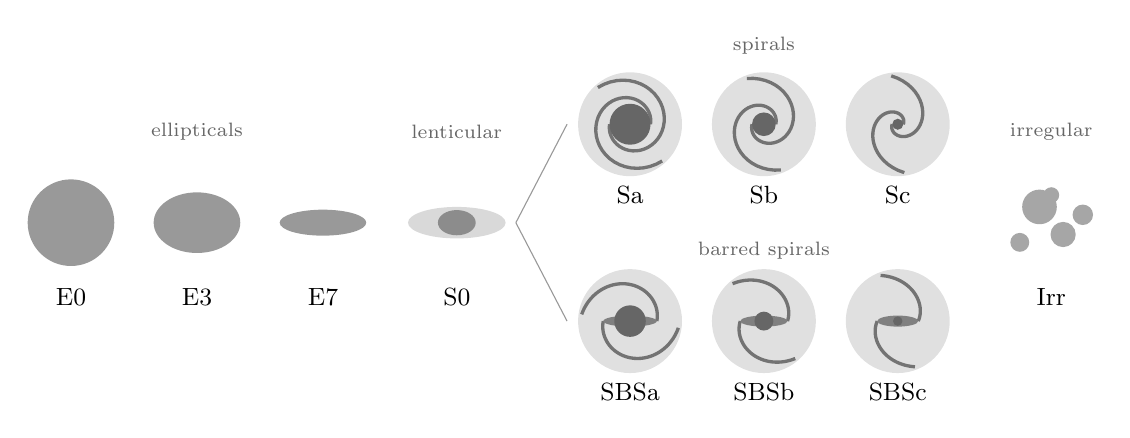
\begin{tikzpicture}[font=\small]
\def\spiralgal#1#2#3#4#5{% x, y, bulge radius, winding rate, bar half-length
  \begin{scope}[shift={(#1,#2)}]
    \fill[black!12] (0,0) circle (0.66);
    \pgfmathsetmacro{\rs}{max(#3,#5)}
    \pgfmathsetmacro{\th}{ln(0.62/\rs)/#4}
    \foreach \a in {0,180}
      \draw[line width=1.2pt, black!55, rotate=\a]
        plot[domain=0:\th, samples=40] ({\rs*exp(#4*\x)*cos(\x r)}, {\rs*exp(#4*\x)*sin(\x r)});
    \ifdim #5pt>0pt \fill[black!50] (0,0) ellipse (#5 and 0.07); \fi
    \fill[black!60] (0,0) circle (#3);
  \end{scope}}
\fill[black!40] (0,0) circle (0.55);
\fill[black!40] (1.6,0) ellipse (0.55 and 0.385);
\fill[black!40] (3.2,0) ellipse (0.55 and 0.165);
\fill[black!15] (4.9,0) ellipse (0.62 and 0.20);
\fill[black!45] (4.9,0) ellipse (0.24 and 0.16);
\draw[black!40] (5.65,0) -- (6.3,1.25);
\draw[black!40] (5.65,0) -- (6.3,-1.25);
\spiralgal{7.1}{1.25}{0.26}{0.16}{0}
\spiralgal{8.8}{1.25}{0.15}{0.28}{0}
\spiralgal{10.5}{1.25}{0.07}{0.45}{0}
\spiralgal{7.1}{-1.25}{0.20}{0.20}{0.34}
\spiralgal{8.8}{-1.25}{0.12}{0.32}{0.30}
\spiralgal{10.5}{-1.25}{0.06}{0.45}{0.26}
\foreach \p/\r in {(12.3,0.2)/0.22,(12.6,-0.15)/0.16,(12.05,-0.25)/0.12,(12.45,0.35)/0.1,(12.85,0.1)/0.13}
  \fill[black!35] \p circle (\r);
\foreach \x/\t in {0/E0,1.6/E3,3.2/E7,4.9/S0}
  \node at (\x,-0.95) {\t};
\foreach \x/\t in {7.1/Sa,8.8/Sb,10.5/Sc}
  { \node at (\x,0.35) {\t}; \node at (\x,-2.15) {SB\t}; }
\node at (12.45,-0.95) {Irr};
\node[font=\scriptsize, black!60] at (1.6,1.15) {ellipticals};
\node[font=\scriptsize, black!60] at (4.9,1.15) {lenticular};
\node[font=\scriptsize, black!60] at (8.8,2.25) {spirals};
\node[font=\scriptsize, black!60] at (8.8,-0.35) {barred spirals};
\node[font=\scriptsize, black!60] at (12.45,1.15) {irregular};
\end{tikzpicture}
\par\smallskip{\small The \omterm{def:b3:milky-way-galaxies:types}{Hubble sequence} drawn as a tuning fork,
schematically. Ellipticals are labelled by their apparent flattening;
the fork branches at the lenticulars into ordinary and barred spirals,
ordered from large bulges and tightly wound arms (a) to small bulges and
open arms (c); irregulars close the sequence.}\label{fig:b3:milky-way-galaxies:fork}
\end{omfigure}
% ledger: buta11:hubble

The classes describe shapes seen on the sky, and a single label hides a
range: an elliptical seen along its shortest axis looks round whatever its
true flattening, and the boundaries between neighbouring classes are a
matter of judgement. In a catalogue of the galaxies near us, the
Galaxy is listed as an S(B)bc, a spiral between Sb and Sc with a bar; its large
neighbour Andromeda (M31) is an Sb, the Triangulum galaxy (M33) an Sc, and
the Large and Small Magellanic Clouds are irregulars.
% ledger: buta11:hubble, mcconn12:local-group

\begin{omfigure}
\centering
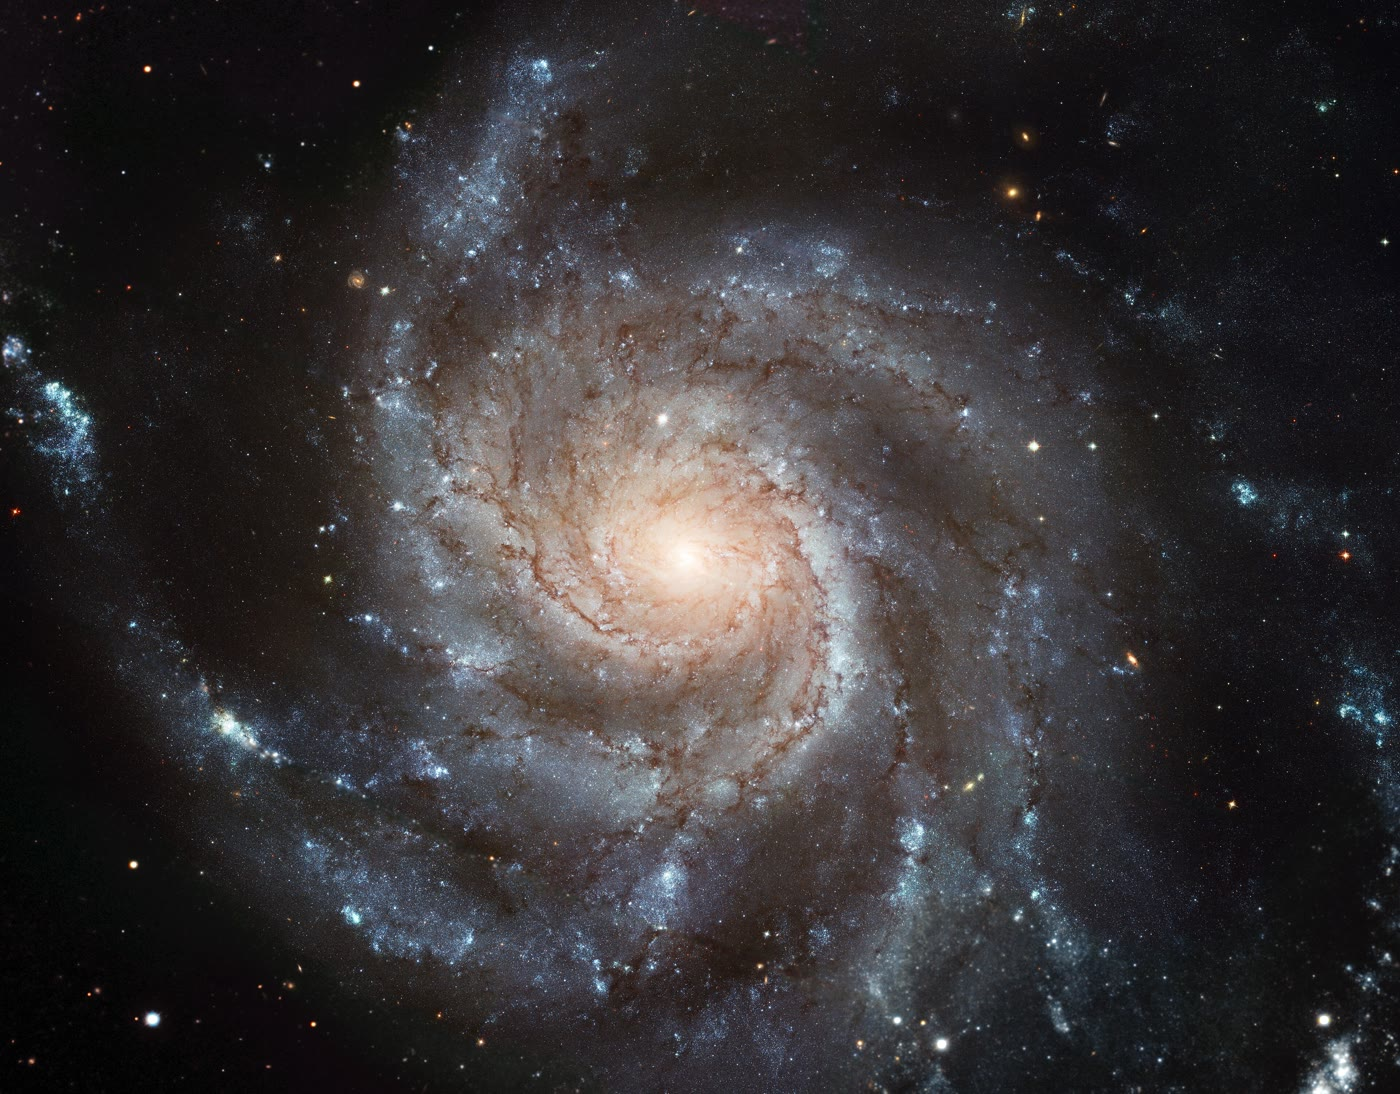
\includegraphics[width=0.66\linewidth]{images/book5/b3-m101.jpg}
\par\smallskip{\small The \omterm{def:b3:milky-way-galaxies:types}{spiral galaxy} M101 seen face-on by the Hubble
Space Telescope, a mosaic of 51 exposures, cropped at its edges: a small,
bright, yellowish bulge; open arms, bluer and knotted with clusters of
young stars; brown lanes of dust along the arms. Image ESA and NASA
(Hubble, heic0602), CC BY~4.0.}\label{fig:b3:milky-way-galaxies:m101}
\end{omfigure}
% ledger: photo:b3-m101

Why are spiral arms not wound up? In a disc whose \omterm{def:b3:milky-way-galaxies:rotation-curve}{rotation curve} is flat,
a star at half the distance from the centre goes round in half the time.
A spiral of stars would wind tighter at each turn, and after a few turns
of the disc it would be a tight coil (\cref{exo:b3:milky-way-galaxies:11}).

\begin{definition}[Density-wave theory]\label{def:b3:milky-way-galaxies:density-wave}
The \emph{density-wave theory}\index{density-wave theory} explains spiral
arms as a wave of higher density in a disc, a spiral pattern that turns
rigidly at its own angular speed, the pattern speed, while the stars and
the gas move through it, slowing as they enter the crowded arm and
speeding up as they leave, as cars move through a traffic jam.
\end{definition}

The theory, proposed in 1964, frees the arms from the winding problem.
Gas entering an arm is compressed, and stars form there: the arms are
picked out by young stars and glowing gas, while the old stars are spread
far more evenly. Whether the arms are long-lived waves is still debated;
computer simulations of discs more often grow arms that are transient,
dissolving and re-forming, and a passing galaxy or a bar can drive a
two-armed spiral.
% ledger: dobbs14:density-wave

\begin{definition}[Supermassive black hole]\label{def:b3:milky-way-galaxies:smbh}
A \emph{supermassive black hole}\index{supermassive black hole} is a black
hole of a million solar masses or more at the centre of a galaxy.
\end{definition}

At the centre of the Galaxy, the compact radio source Sagittarius~A*
(Sgr~A*) sits among stars on tight, fast orbits. Their orbits require a
central mass of about four million suns, $\num[separate-uncertainty=true]{4.2 \pm 0.2 e6}$
solar masses in a review of the measurements. Sgr~A* hardly moves
relative to distant galaxies: once the Sun's orbit is removed, its
residual motion is at most a few kilometres per second, so it holds at
least a quarter of that mass. Its size is comparable to its Schwarzschild
radius, and its density, above \qty{4e23}{} solar masses per cubic
parsec, is very close to that expected of a black hole: the evidence
that Sgr~A* is one is overwhelming.
% ledger: reid20:sgra, bhg16:structure, gravity19:r0

\begin{definition}[Local Group; galaxy cluster]\label{def:b3:milky-way-galaxies:groups}
The \emph{Local Group}\index{Local Group} is the gravitationally bound
group of galaxies dominated by the Milky Way and Andromeda, each with
its satellite galaxies. A \emph{galaxy cluster}\index{galaxy cluster} is
one of the largest gravitationally bound systems: many galaxies held,
with a hot gas that radiates X-rays, in a common well of mostly dark
matter.
\end{definition}

More than a hundred galaxies lie within \qty{3}{Mpc} of the Sun, most of
them dwarfs. The Large Magellanic Cloud is at about \qty{50}{kpc}, Andromeda at
\qty{783}{kpc} and approaching us at \qty{300}{km.s^{-1}}, and the bound
members of the group lie within about \qty{1.06}{Mpc} of its centre of
mass, between the Galaxy and Andromeda, where they turn away from the
expansion of the Universe. Its mass, from the motion of the two big
galaxies towards each other, is of order \qty{5e12}{} solar masses. In a
massive \omterm{def:b3:milky-way-galaxies:groups}{galaxy cluster} the hot gas, at about \qty{e8}{K}, holds about ten
times the mass of the stars; galaxies and gas together are too light for
the depth of the gravitational well, and most of the cluster's mass,
of order \qty{e15}{} solar masses, is dark.
% ledger: mcconn12:local-group, kravtsov12:clusters

\section{The distance ladder}\label{sec:b3:milky-way-galaxies:ladder}

A parallax gives a distance by geometry alone, but parallaxes shrink with
distance. The best catalogue of them measures a parallax with an
uncertainty of 0.02 to \qty{0.03}{mas} for stars brighter than
magnitude~15, so a distance to \qty{10}{\percent} out to about
\qty{4}{kpc}; the Large Magellanic Cloud, at \qty{50}{kpc}, has a
parallax of \qty{0.02}{mas}. Beyond, distances rest on objects whose
luminosity is known.
% ledger: gaia:dr3, freedman19:trgb

\begin{definition}[Standard candle; distance ladder]\label{def:b3:milky-way-galaxies:ladder}
A \emph{standard candle}\index{standard candle} is a class of objects
whose absolute magnitude is known, or can be inferred from a property
measured independently of distance, so that its apparent magnitude gives
its distance modulus. The \emph{distance ladder}\index{distance ladder} is
the chain of methods, each calibrated on objects close enough to be
measured also by the method before it, that carries distances from
parallaxes out to the expanding Universe.
\end{definition}

\begin{definition}[Cepheid variable; Leavitt law]\label{def:b3:milky-way-galaxies:cepheid}
A \emph{Cepheid variable}\index{Cepheid variable} is a young, luminous,
pulsating star whose brightness varies with a strictly regular period,
from about a day to several weeks. The \emph{Leavitt law}\index{Leavitt law},
or period--luminosity relation, is the linear relation between the mean
absolute magnitude of a Cepheid and the logarithm of its period, longer
periods for brighter stars.
\end{definition}

The relation was discovered in the Small Magellanic Cloud, whose stars
are all at nearly the same distance, in 1908. Dust in the galaxy that
hosts a Cepheid dims and reddens it; but the dimming is larger in the
visible than in the near infrared, in a fixed ratio for a given kind of
dust, and the combination $W_I = I - 1.55\,(V - I)$ of the magnitudes in
the I and V bands, the Wesenheit index, is chosen so that the dimming
cancels. The figure below shows it for 2315 Cepheids of the Large
Magellanic Cloud: the \omterm{def:b3:milky-way-galaxies:cepheid}{Leavitt law} is a tight line, with a scatter of
\qty{0.078}{mag}, that is, \qty{3.6}{\percent} in distance for a single
star.
% ledger: sos15:leavitt, data:b5-ogle-lmc-cep

\begin{omfigure}
\centering
\begin{tikzpicture}
\begin{axis}[width=0.80\linewidth, height=0.52\linewidth,
  xmin=-0.05, xmax=1.6, ymin=10, ymax=16.6, y dir=reverse,
  xlabel={$\log_{10}(P/\mathrm{d})$}, ylabel={Wesenheit index $W_I$ (mag)},
  tick label style={font=\scriptsize}, label style={font=\small},
  legend style={font=\scriptsize, at={(0.5,-0.17)}, anchor=north, legend columns=3, draw=none, cells={anchor=west}, /tikz/every even column/.append style={column sep=1em}},
  legend image post style={scale=2.2}]
\addplot[only marks, mark=*, mark size=0.45pt, omDef, opacity=0.6] table[x=logp, y=w] {figdata/out/bachelor-3-distance_ladder-pl.dat};
\addlegendentry{Cepheids}
\addplot[only marks, mark=x, mark size=1.6pt, red!70!black] table[x=logp, y=w] {figdata/out/bachelor-3-distance_ladder-clipped.dat};
\addlegendentry{set aside ($>3\sigma$)}
\addplot[thick, black] table[x=logp, y=w_fit] {figdata/out/bachelor-3-distance_ladder-fit.dat};
\addlegendentry{fit}
\node[font=\scriptsize, anchor=south west, fill=white, inner sep=1pt] at (axis cs:0.55,11.0) {$W_I = -3.315\log_{10}P + 15.889$};
\end{axis}
\end{tikzpicture}
\par\smallskip{\small The \omterm{def:b3:milky-way-galaxies:cepheid}{Leavitt law} in the Large Magellanic Cloud:
the Wesenheit index of 2315 Cepheids pulsating in their fundamental mode
against the logarithm of their period (OGLE survey, Soszy\'nski and
others, 2015, via the CDS). Brighter stars are higher. A straight line
fitted by least squares, after setting aside 92 stars more than three
standard deviations from it, reproduces the published relation
($-3.314$, $15.888$). With the Cloud's distance modulus, 18.477, the line
gives the absolute Wesenheit magnitude of any Cepheid from its period.}\label{fig:b3:milky-way-galaxies:leavitt}
\end{omfigure}
% ledger: data:b5-ogle-lmc-cep, sos15:leavitt, freedman19:trgb

\begin{definition}[Tip of the red giant branch]\label{def:b3:milky-way-galaxies:trgb}
The \emph{tip of the red giant branch}\index{tip of the red giant branch}
(TRGB) is the sharp upper limit of the luminosities of the red giants of
an old \omterm{def:b3:milky-way-galaxies:populations}{stellar population}, set by the ignition of helium in their cores,
the helium flash; in the I band it lies at nearly the same absolute
magnitude in every old population, $M_I \approx -4.05$ at a colour
$V - I = 1.6$, depending only weakly on chemical composition.
\end{definition}

The tip is measured in the sparse haloes of galaxies, where there is
little dust and little crowding; it uses old halo stars where Cepheids use
young disc stars, and the two methods share no physics. Cepheids and the
TRGB reach a few tens of megaparsecs, into galaxies where a rare and far
brighter \omterm{def:b3:milky-way-galaxies:ladder}{standard candle} has gone off: a Type~Ia supernova, the
thermonuclear explosion of a white dwarf recalled from the physics books,
whose peak absolute magnitude, once corrected for the
shape of its light curve and its colour, is
$M_B = \qty[separate-uncertainty=true]{-19.253 \pm 0.027}{mag}$. Such
supernovae are seen across hundreds of megaparsecs.
% ledger: freedman19:trgb, riess22:h0

\begin{definition}[Tully--Fisher relation]\label{def:b3:milky-way-galaxies:tully-fisher}
The \emph{Tully--Fisher relation}\index{Tully--Fisher relation} is the
correlation between the luminosity, or better the mass of stars and gas,
of a \omterm{def:b3:milky-way-galaxies:types}{spiral galaxy} and the speed of its flat \omterm{def:b3:milky-way-galaxies:rotation-curve}{rotation curve}; in its
baryonic form, $M_\mathrm{b} = A\,V^4$, it holds from about 30 to
\qty{300}{km.s^{-1}}.
\end{definition}

The 21-cm spectrum of a galaxy gives its maximum rotation speed, the
relation its luminosity, independently of its distance, and its flux
then gives the distance: a rung for spiral galaxies too far for single
stars. The Galaxy, by its luminosity and rotation, falls on the relation.
% ledger: mcgaugh00:btf, nrao:hi-line, bhg16:structure

\begin{omfigure}
\centering
\pgfplotstableread{figdata/out/bachelor-3-distance_ladder-ladder.dat}\laddertab
\pgfplotstableread{figdata/out/bachelor-3-distance_ladder-anchors.dat}\anchortab
\pgfplotstablegetelem{0}{d_hi}\of{\laddertab}\let\plxhi\pgfplotsretval
\pgfplotstablegetelem{1}{d_lo}\of{\laddertab}\let\cephlo\pgfplotsretval
\pgfplotstablegetelem{1}{d_hi}\of{\laddertab}\let\cephhi\pgfplotsretval
\pgfplotstablegetelem{3}{d_lo}\of{\laddertab}\let\snlo\pgfplotsretval
\pgfplotstablegetelem{3}{d_hi}\of{\laddertab}\let\snhi\pgfplotsretval
\pgfplotstablegetelem{1}{d}\of{\anchortab}\let\mthirtyone\pgfplotsretval
\pgfplotstablegetelem{2}{d}\of{\anchortab}\let\nfourtwo\pgfplotsretval
\begin{tikzpicture}
\begin{axis}[width=0.92\linewidth, height=0.42\linewidth,
  xmode=log, xmin=1e-3, xmax=2e6, ymin=0.4, ymax=4.9,
  ytick={1,2,3,4}, yticklabels={parallaxes, Cepheids, TRGB, SNe~Ia},
  xtick={1e-3,1e-2,1e-1,1,10,100,1e3,1e4,1e5,1e6},
  xticklabels={1~pc,,,1~kpc,,,1~Mpc,,,1~Gpc},
  xlabel={distance}, tick label style={font=\scriptsize}, label style={font=\small},
  y tick label style={font=\small}, axis y line*=left, axis x line*=bottom]
\draw[line width=7pt, omDef!70] (axis cs:1e-3,1) -- (axis cs:\plxhi,1);
\draw[line width=7pt, omMeth!70] (axis cs:\cephlo,2) -- (axis cs:\cephhi,2);
\draw[line width=7pt, omProp!70] (axis cs:\cephlo,3) -- (axis cs:\cephhi,3);
\draw[line width=7pt, red!60] (axis cs:\snlo,4) -- (axis cs:\snhi,4);
\draw[densely dotted, thick] (axis cs:\cephlo,0.4) -- (axis cs:\cephlo,4.55) node[anchor=south, font=\scriptsize] {LMC};
\draw[densely dotted, thick] (axis cs:\mthirtyone,0.4) -- (axis cs:\mthirtyone,4.55) node[anchor=south, font=\scriptsize] {M31};
\draw[densely dotted, thick] (axis cs:\nfourtwo,0.4) -- (axis cs:\nfourtwo,4.55) node[anchor=south, font=\scriptsize] {NGC~4258};
\draw[->, thick, black!60] (axis cs:\plxhi,1.25) to[out=30, in=200] (axis cs:\cephlo,1.75);
\draw[->, thick, black!60] (axis cs:\cephhi,2.25) to[out=40, in=220] (axis cs:\snlo,3.75);
\end{axis}
\end{tikzpicture}
\par\smallskip{\small The rungs of the \omterm{def:b3:milky-way-galaxies:ladder}{distance ladder}, with the
distances over which each is used here: parallaxes of the best catalogue,
to \qty{10}{\percent} out to \qty{4}{kpc}; Cepheids and the TRGB from the
Large Magellanic Cloud to the hosts of the nearest Type~Ia supernovae,
\qty{45}{Mpc}; the supernovae of the smooth expansion, at redshifts 0.023
to 0.15 (\qtyrange{96}{616}{Mpc} for $H_0 = 73$). Dotted: two anchors of
the Cepheid scale with geometric distances (eclipsing binaries in the
LMC, water masers orbiting the black hole of NGC~4258), and M31, the
nearest large spiral. Arrows: each rung is calibrated on objects that the
one below also measures, the Cepheids of the Galaxy by their parallaxes,
the supernovae of nearby galaxies by the Cepheids and the TRGB of their
hosts.}\label{fig:b3:milky-way-galaxies:ladder-rungs}
\end{omfigure}
% ledger: gaia:dr3, riess22:h0, freedman19:trgb, mcconn12:local-group

At the top of the ladder, the supernovae measure the expansion of the
Universe. Hubble's law, recalled from the physics books, makes the
recession speed $cz$ of a distant galaxy proportional to its distance $d$,
$cz = H_0 d$ for small redshifts $z$; the Hubble constant $H_0$ is the
slope, and the supernovae, with their distances from the ladder, give it.

\begin{definition}[Hubble tension]\label{def:b3:milky-way-galaxies:tension}
The \emph{Hubble tension}\index{Hubble tension} is the disagreement
between the value of the Hubble constant measured locally with the
\omterm{def:b3:milky-way-galaxies:ladder}{distance ladder} and the value inferred from the cosmic microwave
background with the standard cosmological model.
\end{definition}

\begin{dated}{2022}
The Cepheids of the hosts of 42 Type~Ia supernovae, anchored on Gaia
parallaxes, the masers of NGC~4258 and the eclipsing binaries of the
Large Magellanic Cloud, give
$H_0 = \qty[separate-uncertainty=true]{73.04 \pm 1.04}{km.s^{-1}.Mpc^{-1}}$.
The \omterm{def:b3:milky-way-galaxies:trgb}{tip of the red giant branch}, calibrating about a hundred supernovae,
gave in 2019 $H_0 = 69.8 \pm 0.8 \pm \qty{1.7}{km.s^{-1}.Mpc^{-1}}$
(statistical and systematic). The Planck satellite's map of the cosmic
microwave background, read with the standard cosmological model, implies
$H_0 = \qty[separate-uncertainty=true]{67.4 \pm 0.5}{km.s^{-1}.Mpc^{-1}}$.
The Cepheid value and the background value differ by five standard
deviations; the TRGB value lies between them. The source of the
discrepancy is not known: an error not yet found in one of the ladders,
or physics missing from the model.
\end{dated}
% ledger: riess22:h0, freedman19:trgb, planck18:h0

\begin{inthelab}[An astrometric satellite and its catalogue]
The satellite Gaia scans the sky along a commanded pattern, so that every
star is measured again and again over the mission. On the ground, the
coordination units of a data-processing consortium turn these
measurements into a position, a parallax and a proper motion for each of
more than a billion sources: of the small motions of a star on the sky,
the parallax is the part that repeats each year and the proper motion
the part that accumulates. Each catalogue is released with papers that
describe its processing and its validation, and every distance in the
figures of this section that rests on a parallax rests on such a
catalogue.
\end{inthelab}

\begin{dated}{2022}
The third Gaia catalogue, released on 13 June 2022 from 34 months of
observations, gives positions, parallaxes and proper motions for about
1.46~billion sources, from magnitude~3 to~21, and mean radial velocities
for 33~million stars. Its parallax uncertainties are 0.02 to
\qty{0.03}{mas} for stars brighter than magnitude~15, \qty{0.07}{mas} at
magnitude~17, and \qty{0.5}{mas} at magnitude~20.
\end{dated}
% ledger: gaia:dr3

\section{Exercises}

\begin{exercise}[$\star$]\label{exo:b3:milky-way-galaxies:1}
The Sun's Galactic year. (a)~With $R_0 = \qty{8.178}{kpc}$ and
$V_0 = \qty{229}{km.s^{-1}}$, compute the period of the Sun's orbit about
the Galactic Centre, in millions of years. (b)~How many times has the Sun
gone round since the Solar System formed, \qty{4.54}{Gyr} ago?
\end{exercise}

\begin{exercise}[$\star$]\label{exo:b3:milky-way-galaxies:2}
The reflex motion of Sgr~A*. (a)~A proper motion of \qty{1}{mas} a year
at \qty{1}{kpc} is a transverse speed of \qty{1}{au} a year: express it in
kilometres per second. (b)~Sgr~A*, assumed at rest at the Galactic Centre
at \qty{8.178}{kpc}, drifts along the Galactic plane by \qty{6.411}{mas}
a year. Compute the Sun's speed about the centre and compare it with the
review value, \qty[separate-uncertainty=true]{248 \pm 3}{km.s^{-1}}. (c)~Subtract the Sun's
peculiar motion in the direction of rotation, \qty{11}{km.s^{-1}}, and
compare with $V_0$ from the \omterm{def:b3:milky-way-galaxies:rotation-curve}{rotation curve}.
\end{exercise}

\begin{exercise}[$\star$]\label{exo:b3:milky-way-galaxies:3}
Classifying ellipticals. (a)~An \omterm{def:b3:milky-way-galaxies:types}{elliptical galaxy}'s isophotes have an
axis ratio of 0.6: give its class. (b)~What axis ratio does an E7 have?
(c)~Why may an E0 galaxy be a flattened system?
\end{exercise}

\begin{exercise}[$\star$]\label{exo:b3:milky-way-galaxies:4}
Anchors. Compute the distances of the Large Magellanic Cloud
($\mu = 18.477$), Andromeda ($\mu = 24.47$) and NGC~4258
($\mu = 29.398$). What parallax would a star of the Cloud have, and why
can the Cloud's distance not be measured by parallaxes?
\end{exercise}

\begin{exercise}[$\star\star$]\label{exo:b3:milky-way-galaxies:5}
From the \omterm{def:b3:milky-way-galaxies:rotation-curve}{Oort constants} $A = \qty{15.3}{km.s^{-1}.kpc^{-1}}$ and
$B = \qty{-11.9}{km.s^{-1}.kpc^{-1}}$: (a)~compute the angular speed of
the LSR and, with $R_0 = \qty{8.178}{kpc}$, the circular velocity $V_0$;
(b)~compute the slope of the \omterm{def:b3:milky-way-galaxies:rotation-curve}{rotation curve} at the Sun. (c)~Compare
with the \omterm{def:b3:milky-way-galaxies:rotation-curve}{rotation curve} of the red giants ($V_0 = \qty{229.0}{km.s^{-1}}$,
slope \qty{-1.7}{km.s^{-1}} per kiloparsec) and suggest why the two
differ, given that the same measurement found non-zero $C$ and $K$.
\end{exercise}

\begin{exercise}[$\star\star$]\label{exo:b3:milky-way-galaxies:6}
A flat \omterm{def:b3:milky-way-galaxies:rotation-curve}{rotation curve} and the local density. (a)~For a spherical galaxy
with a flat \omterm{def:b3:milky-way-galaxies:rotation-curve}{rotation curve} at \qty{229}{km.s^{-1}}, compute the density at
\qty{8.178}{kpc}, in solar masses per cubic parsec
($G = \qty{4.301e-6}{kpc.(km.s^{-1})^2}$ per solar mass). (b)~Show that
one solar mass per cubic parsec is \qty{37.96}{GeV.cm^{-3}}, and express
the local dark-matter density, \qty{0.30}{GeV.cm^{-3}}, in solar masses
per cubic parsec. (c)~Why is the density of (a) larger?
\end{exercise}

\begin{exercise}[$\star\star$]\label{exo:b3:milky-way-galaxies:7}
A Cepheid distance. In an invented \omterm{def:b3:milky-way-galaxies:types}{spiral galaxy} a Cepheid of period
\qty{30}{d} has a mean Wesenheit index $W_I = \qty{25.00}{mag}$.
(a)~Using the \omterm{def:b3:milky-way-galaxies:cepheid}{Leavitt law} of the Large Magellanic Cloud,
$W_I = -3.314\log_{10}P + 15.888$, and the Cloud's distance modulus
18.477, compute the Cepheid's absolute Wesenheit magnitude. (b)~Compute
the galaxy's distance. (c)~The law's scatter is \qty{0.077}{mag}: what is
the relative distance error from one Cepheid, and from fifty?
\end{exercise}

\begin{exercise}[$\star\star$]\label{exo:b3:milky-way-galaxies:8}
A TRGB distance. In the halo of an invented galaxy the \omterm{def:b3:milky-way-galaxies:trgb}{tip of the red
giant branch} is found at $I = \qty{26.00}{mag}$; the dust along the line of
sight dims the I band by \qty{0.05}{mag}. With $M_I = -4.05$, compute the
distance modulus and the distance. What does an uncertainty of
\qty{0.04}{mag} on the tip mean in distance?
\end{exercise}

\begin{exercise}[$\star\star$]\label{exo:b3:milky-way-galaxies:9}
The Hubble constant from supernovae. For a supernova of the smooth
expansion, $\log_{10}(cz) - 0.2\,m_B = a_B$, the intercept of the
supernovae's Hubble diagram, and the distance modulus is
$m_B - M_B = 5\log_{10}(d/\mathrm{Mpc}) + 25$. (a)~Show that
$\log_{10}H_0 = 0.2\,M_B + a_B + 5$ ($H_0$ in kilometres per second per
megaparsec). (b)~With $M_B = -19.253$ and $a_B = 0.714158$, compute $H_0$.
(c)~What $M_B$ would give $H_0 = \qty{67.4}{km.s^{-1}.Mpc^{-1}}$? By how
many magnitudes, and by what fraction of the distances, do the two
calibrations differ?
\end{exercise}

\begin{exercise}[$\star\star\star$]\label{exo:b3:milky-way-galaxies:10}
Where the Tully--Fisher law comes from. (a)~A disc galaxy of mass $M$
and radius $R$ rotates at $V$: show that $M \approx RV^2/G$. (b)~If all
spiral galaxies had the same mean surface density $\Sigma = M/(\pi R^2)$,
show that $M \propto V^4$. (c)~Two invented galaxies on the same baryonic
relation rotate at 100 and \qty{229}{km.s^{-1}}: what is the ratio of
their masses? (d)~Two galaxies rotate at the same speed and have the same
luminosity; one gives four times the flux of the other. Compare their
distances.
\end{exercise}

\begin{exercise}[$\star\star\star$]\label{exo:b3:milky-way-galaxies:11}
The winding problem. A disc rotates with a flat curve at
\qty{229}{km.s^{-1}}. (a)~Convert this speed to kiloparsecs per billion
years. (b)~A straight arm of stars runs at time zero from 4 to
\qty{12}{kpc}. Compute the orbital periods at both ends. (c)~After
\qty{1}{Gyr}, by what angle has its inner end gone ahead of its outer
end? How many turns of a spiral is that, and what would the arm look
like? (d)~How does a density wave avoid this?
\end{exercise}

\begin{exercise}[$\star\star\star$]\label{exo:b3:milky-way-galaxies:12}
The black hole at the centre. Take the central mass to be
\qty{4.2e6}{} solar masses and $R_0 = \qty{8178}{pc}$. (a)~The star S2
orbits it in \num{16}~years: compute the semi-major axis of its orbit in
astronomical units (Kepler's third law in solar units, $a^3 = MP^2$ with
$a$ in au, $P$ in years and $M$ in solar masses) and its angular size seen
from the Earth. (b)~Compute the Schwarzschild radius of the black hole in
metres and in astronomical units, and the angle that its diameter
subtends from the Earth, in microarcseconds. (c)~Compute the mean density
of the mass within its Schwarzschild radius, in solar masses per cubic
parsec, and compare it with the lower bound set by the motion of Sgr~A*,
\qty{4e23}{} solar masses per cubic parsec.
\end{exercise}

\section{Problem: Weighing the Galaxy}

\begin{problem}[{Weekend problem --- from the motions of stars and gas to
the dark matter within \qty{20}{kpc}}]
\label{pb:b3:milky-way-galaxies:1}
Take $R_0 = \qty{8.18}{kpc}$, $G = \qty{4.301e-6}{kpc.(km.s^{-1})^2}$ per
solar mass, and \qty{4.74}{km.s^{-1}} for a proper motion of
\qty{1}{mas} a year at \qty{1}{kpc}. All velocities are relative to the
LSR. Use the Oort and tangent-point theorems of the chapter, and the
spherical approximation $M = RV^2/G$ for dynamical masses.

\medskip\noindent\textbf{Part I --- The local rotation.} An invented
survey of red-clump stars, all at $d = \qty{1.00}{kpc}$ in the Galactic
plane, gives a mean radial velocity of \qty{+15.4}{km.s^{-1}} at
$\ell = \ang{45}$ and \qty{-15.2}{km.s^{-1}} at $\ell = \ang{135}$, and
mean proper motions in longitude of \qty{-5.91}{mas} a year at
$\ell = \ang{90}$ and \qty{+0.55}{mas} a year at $\ell = \ang{0}$.
\begin{enumerate}
\item What does Oort's formula predict for the radial velocities at
  $\ell = \ang{45}$, \ang{90}, \ang{135} and \ang{180}?
\item Compute $A$ from the two radial velocities.
\item Compute $B$ from the proper motion at $\ell = \ang{90}$.
\item Compute $B$ again from the proper motion at $\ell = \ang{0}$, and
  compare.
\item Compute the angular speed of the LSR and the circular velocity
  $V_0$.
\item Compute the slope of the \omterm{def:b3:milky-way-galaxies:rotation-curve}{rotation curve} at the Sun. Is the curve
  rising, flat or falling?
\item Compute the period of the Sun's orbit and the number of turns in
  \qty{4.54}{Gyr}.
\end{enumerate}

\medskip\noindent\textbf{Part II --- The inner rotation curve.} Take
$V_0 = \qty{229}{km.s^{-1}}$. The highest radial velocities in the
21-cm profiles at $\ell = \ang{40}$, \ang{50}, \ang{60} and \ang{70} are
82.9, 55.6, 32.4 and \qty{14.9}{km.s^{-1}}.
\begin{enumerate}[resume]
\item Why does the tangent-point method need $\ang{0} < \ell < \ang{90}$
  (or the mirror quadrant), and why does it fail beyond the solar circle?
\item Compute the radius of the tangent point for each longitude.
\item Compute $V(R)$ at each tangent point.
\item By how much, in kilohertz, is the line of the gas at the tangent
  point at $\ell = \ang{40}$ shifted from its rest frequency,
  \qty{1420.405751}{MHz}, and in which direction?
\item Compare with the red-giant curve, which gives \qty{226.8}{km.s^{-1}}
  at \qty{5.27}{kpc} and \qty{229.6}{km.s^{-1}} at \qty{7.22}{kpc}. Is the
  inner curve rising, flat or falling?
\item If the speed at the tangent point at $\ell = \ang{40}$ were that of
  a point mass at the centre carrying the Sun at $V_0$, what would it be?
  What does the comparison say about the distribution of the mass?
\end{enumerate}

\medskip\noindent\textbf{Part III --- The visible mass.} Use the mass
model of the chapter, in units of solar masses and kiloparsecs: a
Plummer bulge $M = \num{1.067e10}$, $b = 0.3$; a thin Miyamoto--Nagai disc
$M = \num{3.944e10}$, $a = 5.3$, $b = 0.25$; a thick one of the same
mass with $a = 2.6$, $b = 0.8$.
\begin{enumerate}[resume]
\item Compute the total visible mass of the model and compare it with the
  review value of the Galaxy's stellar mass, \qty[separate-uncertainty=true]{5 \pm 1 e10}{} solar
  masses.
\item Compute the circular velocity of the bulge alone at \qty{20}{kpc}.
\item Compute those of the thin and of the \omterm{def:b3:milky-way-galaxies:structure}{thick disc} at \qty{20}{kpc}.
\item Compute the circular velocity of all the visible mass at
  \qty{20}{kpc}.
\item Compute the same at $R_0$, and compare with $V_0$.
\item If all the visible mass were concentrated at the centre, what would
  the velocity be at \qty{20}{kpc}? Why is the model's value close to it?
\end{enumerate}

\medskip\noindent\textbf{Part IV --- The dark matter.} The red giants
give a circular velocity of \qty{200}{km.s^{-1}} at \qty{20}{kpc}.
\begin{enumerate}[resume]
\item Compute the dynamical mass within \qty{20}{kpc}.
\item Compute the dynamical mass of the visible matter within
  \qty{20}{kpc}.
\item Compute the mass of dark matter within \qty{20}{kpc}, and show that
  its fraction is $1 - (V_\mathrm{vis}/V)^2$.
\item The NFW halo fitted to the whole curve has
  $\rho_0 = \num{1.06e7}$ solar masses per cubic kiloparsec and
  $R_s = \qty{14.8}{kpc}$. Compute its mass within \qty{20}{kpc} and the
  dark fraction it implies. Why does it differ from the previous answer?
\item Compute the density of that halo at $R_0$, in solar masses per
  cubic parsec and in \unit{GeV.cm^{-3}} (one solar mass per cubic parsec
  is \qty{37.96}{GeV.cm^{-3}}).
\item Give the dark-matter fraction of the mass within \qty{20}{kpc}
  found from the measured velocity, in per cent, to two significant
  figures.
\end{enumerate}
\end{problem}
% ledger: gravity19:r0, eilers19:table1, pouliasis17:model1, eilers19:halo, bhg16:structure, nrao:hi-line, const:G, const:au, iau:parsec, usgs:age-earth
